%%%%%%%%%%%%%%%%%%%%%%%%%%%%%%%%%%%%%%%%%
% University/School Laboratory Report
% LaTeX Template
% Version 3.1 (25/3/14)
%
% This template has been downloaded from:
% http://www.LaTeXTemplates.com
%
% Original author:
% Linux and Unix Users Group at Virginia Tech Wiki 
% (https://vtluug.org/wiki/Example_LaTeX_chem_lab_report)
%
% License:
% CC BY-NC-SA 3.0 (http://creativecommons.org/licenses/by-nc-sa/3.0/)
%
%%%%%%%%%%%%%%%%%%%%%%%%%%%%%%%%%%%%%%%%%

%----------------------------------------------------------------------------------------
%	PACKAGES AND DOCUMENT CONFIGURATIONS
%----------------------------------------------------------------------------------------

\documentclass{article}

\usepackage{graphicx} % Required for the inclusion of images
\usepackage{natbib} % Required to change bibliography style to APA
\usepackage{amsmath} % Required for some math elements 
\usepackage{amsthm}
\usepackage[hyphens]{url}
\usepackage{hyperref}
\usepackage{subcaption}
\usepackage{float}
\usepackage{array}
\usepackage{amssymb}
\usepackage{calrsfs}
\usepackage{pgfplots}
\pgfplotsset{width=10cm,compat=1.9}
\usepackage{bytefield}


\setlength\parindent{0pt} % Removes all indentation from paragraphs

\newtheorem*{remark}{Theorem}
\newtheorem*{definition}{Definition}

%----------------------------------------------------------------------------------------
%	DOCUMENT INFORMATION
%----------------------------------------------------------------------------------------

\title{Homework \#5 \\Telegram vs WhatsApp Security \\[0.2em]\small{}CNS Course Sapienza} % Title and subtitle

\author{Riccardo \textsc{Prinzivalle}, 1904064} % Author name

\date{November 30, 2020} % Date for the report

\begin{document}

\maketitle % Insert the title, author and date

%----------------------------------------------------------------------------------------
%	SECTION 0
%----------------------------------------------------------------------------------------

\section{Homework Goal}

This homework contains a comparison of Telegram and WhatsApp security, with an in deep to protocols comparisons and past and some current threat an vulnerabilities.

%----------------------------------------------------------------------------------------
%	SECTION 1
%----------------------------------------------------------------------------------------

\section{Telegram Security basics}

Telegram uses a security protocol called MTProto, developed by the telegram team. It is a symmetric encryption protocol based on 256-bit symmetric AES encryption, 2048-bit RSA encryption and Diffie–Hellman key exchange. The protocol is divided in 3 layers:

\begin{itemize}
	\item \textbf{High-level} component which defines the method whereby API queries and responses are converted to binary messages.
	\item  \textbf{Cryptographic/authorization} layer which defines the method used to encrypt messages prior to being transmitted through the transport protocol.
	\item  \textbf{Transport} component, which defines the method for the client and the server to transmit messages over some other existing network protocol.
\end{itemize}

\begin{figure}[H]
	\centering
	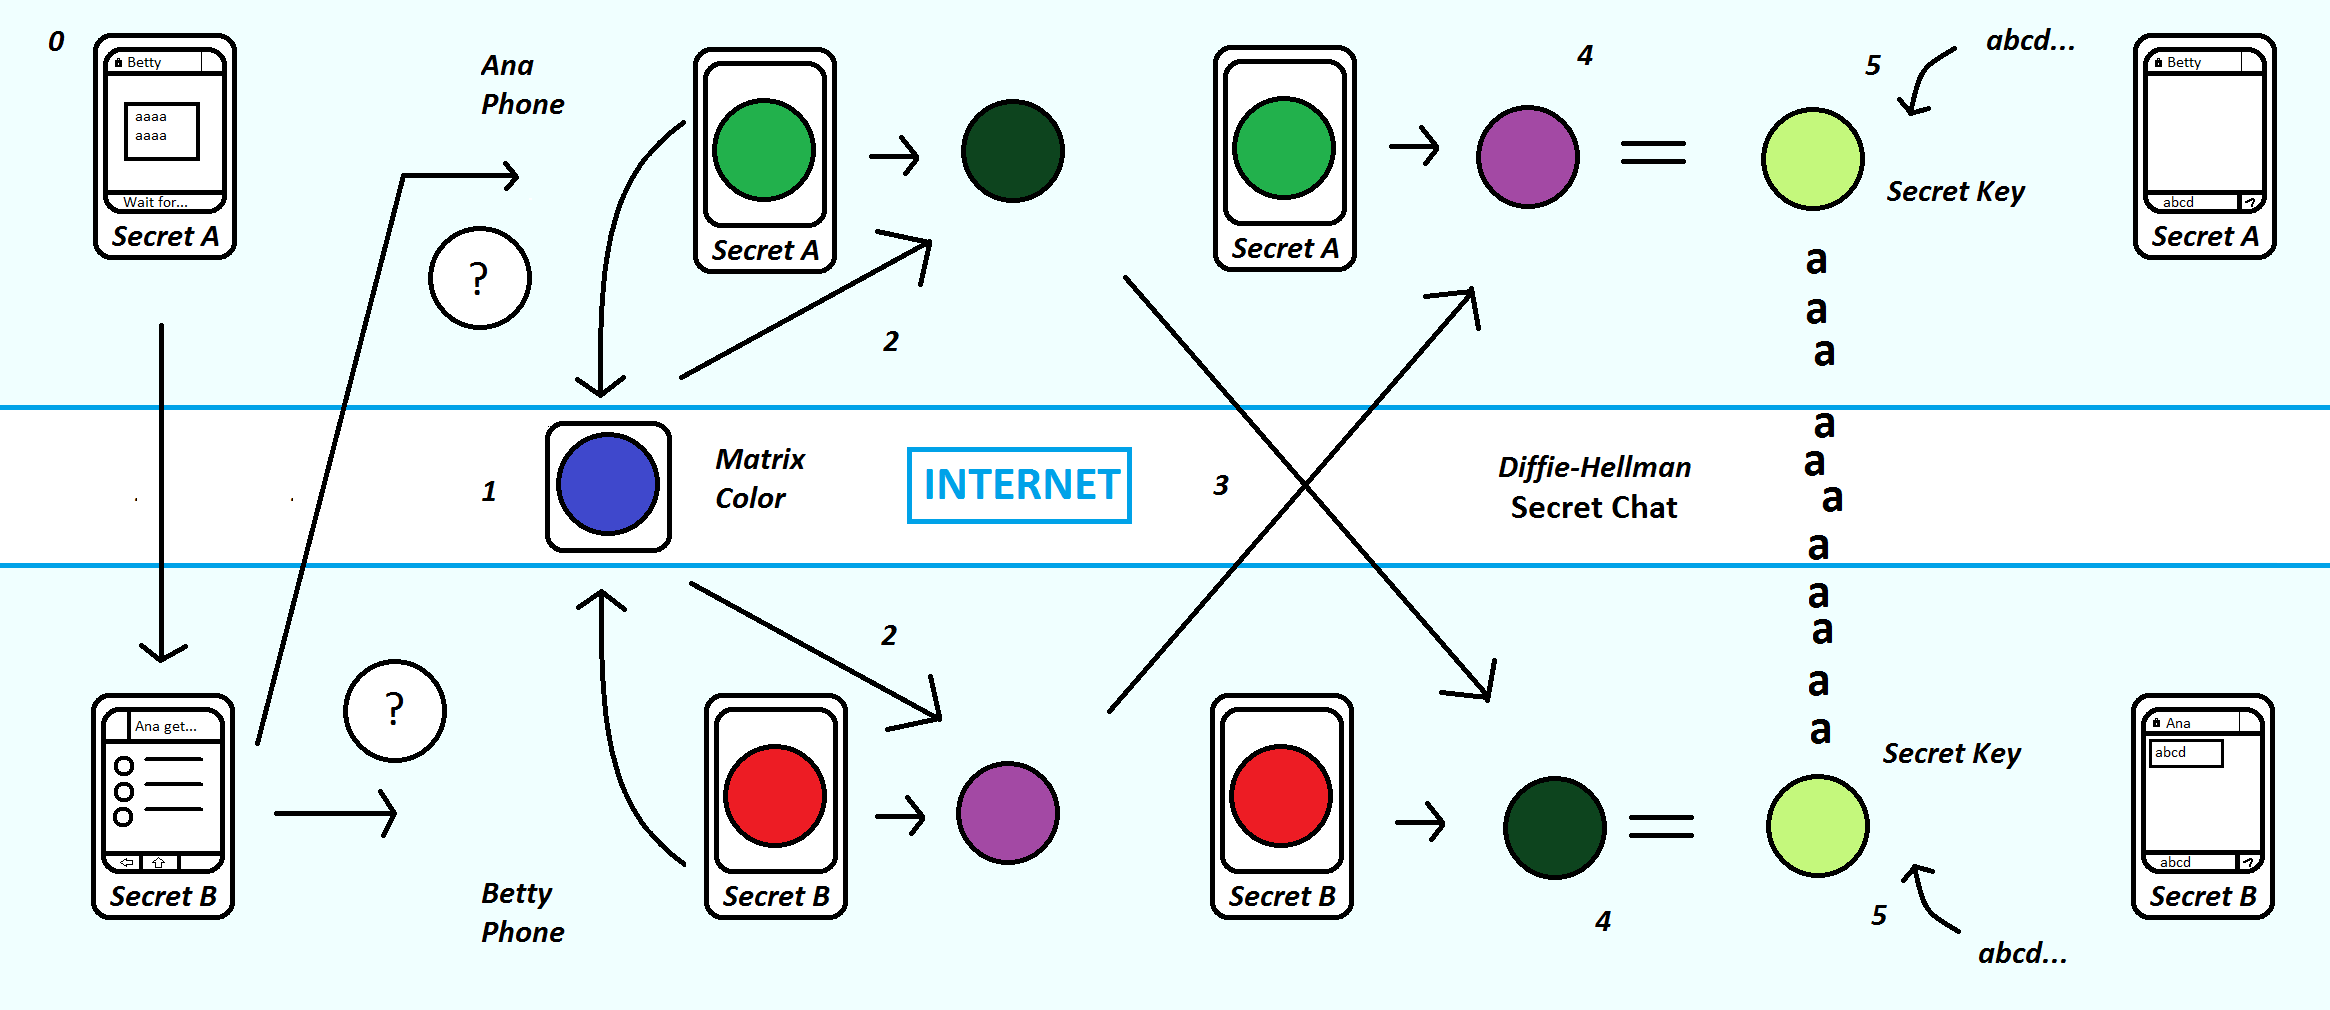
\includegraphics[width=0.9\textwidth]{images/Explanation_of_secret_chats_(Telegram)}
	\caption{Telegram encryption scheme \cite{tel_scheme}}
	\label{fig:LR_graph}
\end{figure}

%----------------------------------------------------------------------------------------
%	SECTION 3
%----------------------------------------------------------------------------------------

\section{WhatsApp Security Basics}



%----------------------------------------------------------------------------------------
%	SECTION 4
%----------------------------------------------------------------------------------------

\section{Protocols comparison}


 
%----------------------------------------------------------------------------------------
%	SECTION 5
%----------------------------------------------------------------------------------------

\section{Past Evolution and Fixed Vulnerabilities}



%----------------------------------------------------------------------------------------
%	SECTION 6
%----------------------------------------------------------------------------------------

\section{Current Vulnerabilities and Security Threats}

%----------------------------------------------------------------------------------------
%	SECTION 7
%----------------------------------------------------------------------------------------

\section{Conclusion}

After this brief introduction on elliptic curves, it is obvious why they have been widely adopted in many cases of asymmetric encryption: they use less bits for the same level of security, so are more efficient to compute and their base concepts are easier to visualize. As suggested on section , EC can be easily used in hybrid encryption scheme, in the key exchange phase.

%----------------------------------------------------------------------------------------
%	BIBLIOGRAPHY
%----------------------------------------------------------------------------------------

\bibliographystyle{abbrv}

\bibliography{biblio}

%----------------------------------------------------------------------------------------


\end{document}